% move all configuration stuff into includes file so we can focus on the content
\documentclass[aspectratio=169,hyperref={pdfpagelabels=false,colorlinks=true,linkcolor=white,urlcolor=blue},t]{beamer}

%%%%%%%%%%%%%%%%%%%%%%%%%%%%%%%%%%%%%%%%%%%%%%%%%%%%%%%%%%%%%%%%%%%%%%%%%%%%%%%%%%
%%%%%%%%%%%%%%%%%%%%%%%%%%%%%%%%%%%%%%%%%%%%%%%%%%%%%%%%%%%%%%%%%%%%%%%%%%%%%%%%%%
% packages
\usepackage{pict2e}
\usepackage{epic}
\usepackage{amsmath,amsfonts,amssymb}
\usepackage{units}
\usepackage{fancybox}
\usepackage[absolute,overlay]{textpos} 
\usepackage{media9} % avi2flv: "C:\Program Files\ffmpeg\bin\ffmpeg.exe" -i TuneFreqFilterbank.avi -b 600k -s 441x324 -r 15 -acodec copy TuneFreqFilterbank.flv
\usepackage{animate}
\usepackage{gensymb}
\usepackage{multirow}
\usepackage{silence}
\usepackage{tikz}
\usepackage[backend=bibtex,style=ieee]{biblatex}
\AtEveryCitekey{\iffootnote{\tiny}{}}
\addbibresource{include/references}

%%%%%%%%%%%%%%%%%%%%%%%%%%%%%%%%%%%%%%%%%%%%%%%%%%%%%%%%%%%%%%%%%%%%%%%%%%%%%%%%%%
%%%%%%%%%%%%%%%%%%%%%%%%%%%%%%%%%%%%%%%%%%%%%%%%%%%%%%%%%%%%%%%%%%%%%%%%%%%%%%%%%%
% relative paths
\graphicspath{{graph/}}


%%%%%%%%%%%%%%%%%%%%%%%%%%%%%%%%%%%%%%%%%%%%%%%%%%%%%%%%%%%%%%%%%%%%%%%%%%%%%%%%%%
%%%%%%%%%%%%%%%%%%%%%%%%%%%%%%%%%%%%%%%%%%%%%%%%%%%%%%%%%%%%%%%%%%%%%%%%%%%%%%%%%%
% units
\setlength{\unitlength}{1mm}

%%%%%%%%%%%%%%%%%%%%%%%%%%%%%%%%%%%%%%%%%%%%%%%%%%%%%%%%%%%%%%%%%%%%%%%%%%%%%%%%%%
%%%%%%%%%%%%%%%%%%%%%%%%%%%%%%%%%%%%%%%%%%%%%%%%%%%%%%%%%%%%%%%%%%%%%%%%%%%%%%%%%%
% theme & layout
\usetheme{Frankfurt}
\beamertemplatenavigationsymbolsempty
%\setbeamertemplate{frametitle}[smoothbars theme]
\setbeamertemplate{frametitle}
{
    \begin{beamercolorbox}[ht=1.8em,wd=\paperwidth]{frametitle}
        \vspace{-.1em}%
        \hspace{.2em}{\strut\insertframetitle\strut}
        
        \hspace{.2em}\small\strut\insertframesubtitle\strut
        %\hfill
        %\includegraphics[height=.8cm,keepaspectratio]{CenterMusicTechnology-solid-2lines-white-CoAtag}
        
    \end{beamercolorbox}
    \begin{textblock*}{100mm}(11.6cm,.7cm)
        \includegraphics[height=.8cm,keepaspectratio]{Logo_GTCMT_black}
    \end{textblock*}
}
\setbeamertemplate{footline}[frame number]

% set this to ensure bulletpoints without subsections
\usepackage{remreset}
\makeatletter
\@removefromreset{subsection}{section}
\makeatother
\setcounter{subsection}{1}

%---------------------------------------------------------------------------------
% appearance
\setbeamercolor{structure}{fg=gtgold}
\setbeamercovered{transparent} %invisible
\setbeamercolor{bibliography entry author}{fg=black}
\setbeamercolor*{bibliography entry title}{fg=black}
\setbeamercolor*{bibliography entry note}{fg=black}
\setbeamercolor{frametitle}{fg=black}
\setbeamercolor{title}{fg=black}

%\usepackage{pgfpages}
%\setbeameroption{show notes}
%\setbeameroption{show notes on second screen=right}
%---------------------------------------------------------------------------------
% fontsize
\let\Tiny=\tiny

%%%%%%%%%%%%%%%%%%%%%%%%%%%%%%%%%%%%%%%%%%%%%%%%%%%%%%%%%%%%%%%%%%%%%%%%%%%%%%%%%%
%%%%%%%%%%%%%%%%%%%%%%%%%%%%%%%%%%%%%%%%%%%%%%%%%%%%%%%%%%%%%%%%%%%%%%%%%%%%%%%%%%
% warnings
\pdfsuppresswarningpagegroup=1
\WarningFilter{biblatex}{Patching footnotes failed}
\WarningFilter{latexfont}{Font shape}
\WarningFilter{latexfont}{Some font shapes}
\WarningFilter{gensymb}{Not defining}


%%%%%%%%%%%%%%%%%%%%%%%%%%%%%%%%%%%%%%%%%%%%%%%%%%%%%%%%%%%%%%%%%%%%%%%%%%%%%%%%%%
%%%%%%%%%%%%%%%%%%%%%%%%%%%%%%%%%%%%%%%%%%%%%%%%%%%%%%%%%%%%%%%%%%%%%%%%%%%%%%%%%%
% theme & layout
\usetheme{Frankfurt}
\useinnertheme{rectangles}


%%%%%%%%%%%%%%%%%%%%%%%%%%%%%%%%%%%%%%%%%%%%%%%%%%%%%%%%%%%%%%%%%%%%%%%%%%%%%%%%%%
\setbeamertemplate{frametitle}[default][colsep=-4bp,rounded=false,shadow=false]
\setbeamertemplate{frametitle}
{%
    \nointerlineskip%
    %\vskip-0.5ex
    \begin{beamercolorbox}[wd=\paperwidth,ht=3.5ex,dp=0.6ex]{frametitle}
        \hspace*{1.3ex}\insertframetitle%
        
        \hspace*{1.3ex}\small\insertframesubtitle%
    \end{beamercolorbox}%
    \begin{textblock*}{100mm}(11.6cm,.57cm)
        
\includegraphics[height=.8cm,keepaspectratio]{graph/Logo_GTCMT_white}
    \end{textblock*}
}


%%%%%%%%%%%%%%%%%%%%%%%%%%%%%%%%%%%%%%%%%%%%%%%%%%%%%%%%%%%%%%%%%%%%%%%%%%%%%%%%%%
\setbeamertemplate{title page}[default][colsep=-4bp,rounded=false,shadow=false]
\setbeamertemplate{title page}
{
    \begin{textblock*}{100mm}(15cm,.51cm)
            \href{https://github.com/alexanderlerch/ACA-Slides/blob/2nd_edition/\jobname.pdf}{\includegraphics[height=.5cm,keepaspectratio]{graph/Logo_github}}\hspace*{2ex}
    \end{textblock*}
    \vskip-10ex
    \begin{beamercolorbox}[wd=\paperwidth,ht=.7\paperheight,dp=0.6ex]{frametitle} %35ex
        %\begin{flushright}
            %\href{http://www.gtcmt.gatech.edu}{\includegraphics[height=.8cm,keepaspectratio]{graph/Logo_GTCMT_black}}\hspace*{2ex}
        %\end{flushright}
        
        \hspace*{1.8ex}\LARGE\inserttitle%
        
        \vspace*{.5ex}
        
        \hspace*{1.3ex}\small\insertsubtitle%
        
        \vspace*{.5ex}
    \end{beamercolorbox}%
    \nointerlineskip%
    \begin{beamercolorbox}[wd=\paperwidth,ht=.4\paperheight,dp=0.6ex]{page number in head/foot}
        %\vspace*{-.5ex}
        \hspace*{1.7ex}\small\insertauthor%
        
        %\hspace*{1.7ex}\small }%
        
        \vspace*{10ex}
        
        \begin{flushright}
            \href{http://www.gtcmt.gatech.edu}{\includegraphics[height=.8cm,keepaspectratio]{graph/Logo_GTCMT_black}}\hspace*{2ex}
        \end{flushright}
    \end{beamercolorbox}%
}


%%%%%%%%%%%%%%%%%%%%%%%%%%%%%%%%%%%%%%%%%%%%%%%%%%%%%%%%%%%%%%%%%%%%%%%%%%%%%%%%%%
%\makeatother
\setbeamertemplate{footline}
{
  \leavevmode%
  \hbox{%
  \begin{beamercolorbox}[wd=.5\paperwidth,ht=2.25ex,dp=1ex,left,leftskip=1ex]{page number in head/foot}%
    \insertsubtitle
  \end{beamercolorbox}%
  \begin{beamercolorbox}[wd=.5\paperwidth,ht=2.25ex,dp=1ex,right,rightskip=1ex]{page number in head/foot}%
    \hfill
    \insertframenumber{} / \inserttotalframenumber
  \end{beamercolorbox}}%
  \vskip0pt%
}
%\makeatletter


%%%%%%%%%%%%%%%%%%%%%%%%%%%%%%%%%%%%%%%%%%%%%%%%%%%%%%%%%%%%%%%%%%%%%%%%%%%%%%%%%%
\beamertemplatenavigationsymbolsempty
\setbeamertemplate{navigation symbols}{}
\setbeamertemplate{blocks}[default]%[rounded=false,shadow=false]
\setbeamertemplate{itemize item}[square]
\setbeamertemplate{itemize subitem}[circle]
\setbeamertemplate{itemize subsubitem}[triangle]
\setbeamertemplate{enumerate item}[square]
\setbeamertemplate{enumerate subitem}[circle]
\setbeamertemplate{enumerate subsubitem}[circle]


%%%%%%%%%%%%%%%%%%%%%%%%%%%%%%%%%%%%%%%%%%%%%%%%%%%%%%%%%%%%%%%%%%%%%%%%%%%%%%%%%%
% colors
\setbeamercolor{structure}{fg=darkgray}
\setbeamercovered{transparent} %invisible
\setbeamercolor{bibliography entry author}{fg=black}
\setbeamercolor*{bibliography entry title}{fg=black}
\setbeamercolor*{bibliography entry note}{fg=black}
\setbeamercolor{frametitle}{fg=black}
\setbeamercolor{title}{fg=white}
\setbeamercolor{subtitle}{fg=white}
\setbeamercolor{frametitle}{fg=white}
\setbeamercolor{framesubtitle}{fg=white}
\setbeamercolor{mini frame}{fg=white, bg=black}
\setbeamercolor{section in head/foot}{fg=white, bg=darkgray}
\setbeamercolor{page number in head/foot}{fg=black, bg=lightblue}
\setbeamercolor{item projected}{fg=white, bg=black}

%---------------------------------------------------------------------------------
%%%%%%%%%%%%%%%%%%%%%%%%%%%%%%%%%%%%%%%%%%%%%%%%%%%%%%%%%%%%%%%%%%%%%%%%%%%%%%%%%%
%%%%%%%%%%%%%%%%%%%%%%%%%%%%%%%%%%%%%%%%%%%%%%%%%%%%%%%%%%%%%%%%%%%%%%%%%%%%%%%%%%
% title information
\title[]{Introduction to \textbf{Audio Content Analysis}}   
\author[alexander lerch]{alexander lerch} 
%\institute{~}
%\date[Alexander Lerch]{}
%\titlegraphic{\vspace{-16mm}\includegraphics[width=\textwidth,height=3cm]{title}}

%%%%%%%%%%%%%%%%%%%%%%%%%%%%%%%%%%%%%%%%%%%%%%%%%%%%%%%%%%%%%%%%%%%%%%%%%%%%%%%%%%
%%%%%%%%%%%%%%%%%%%%%%%%%%%%%%%%%%%%%%%%%%%%%%%%%%%%%%%%%%%%%%%%%%%%%%%%%%%%%%%%%%
% colors
\definecolor{gtgold}{HTML}{E0AA0F} %{rgb}{0.88,0.66,1,0.06} [234, 170, 0]/256
\definecolor{darkgray}{rgb}{.1, .1, .25}
\definecolor{lightblue}{rgb}{.1, 0.75, 1}
\definecolor{highlight}{rgb}{0, 0, 1} %_less!40

%%%%%%%%%%%%%%%%%%%%%%%%%%%%%%%%%%%%%%%%%%%%%%%%%%%%%%%%%%%%%%%%%%%%%%%%%%%%%%%%%%
%%%%%%%%%%%%%%%%%%%%%%%%%%%%%%%%%%%%%%%%%%%%%%%%%%%%%%%%%%%%%%%%%%%%%%%%%%%%%%%%%%
% relative paths
\graphicspath{{../ACA-Plots/graph/}}


%%%%%%%%%%%%%%%%%%%%%%%%%%%%%%%%%%%%%%%%%%%%%%%%%%%%%%%%%%%%%%%%%%%%%%%%%%%%%%%%%%
%%%%%%%%%%%%%%%%%%%%%%%%%%%%%%%%%%%%%%%%%%%%%%%%%%%%%%%%%%%%%%%%%%%%%%%%%%%%%%%%%%
% units
\setlength{\unitlength}{1mm}

%%%%%%%%%%%%%%%%%%%%%%%%%%%%%%%%%%%%%%%%%%%%%%%%%%%%%%%%%%%%%%%%%%%%%%%%%%%%%%%%%%
%%%%%%%%%%%%%%%%%%%%%%%%%%%%%%%%%%%%%%%%%%%%%%%%%%%%%%%%%%%%%%%%%%%%%%%%%%%%%%%%%%
% math
\DeclareMathOperator*{\argmax}{argmax}
\DeclareMathOperator*{\argmin}{argmin}
\DeclareMathOperator*{\atan}{atan}
\DeclareMathOperator*{\arcsinh}{arcsinh}
\DeclareMathOperator*{\sign}{sign}
\DeclareMathOperator*{\tcdf}{tcdf}
\DeclareMathOperator*{\si}{sinc}
\DeclareMathOperator*{\princarg}{princarg}
\DeclareMathOperator*{\arccosh}{arccosh}
\DeclareMathOperator*{\hwr}{HWR}
\DeclareMathOperator*{\flip}{flip}
\DeclareMathOperator*{\sinc}{sinc}
\DeclareMathOperator*{\floor}{floor}
\newcommand{\e}{{e}}
\newcommand{\jom}{\mathrm{j}\omega}
\newcommand{\jOm}{\mathrm{j}\Omega}
\newcommand   {\mat}[1]    		{\boldsymbol{\uppercase{#1}}}		%bold
\renewcommand {\vec}[1]    		{\boldsymbol{\lowercase{#1}}}		%bold

%%%%%%%%%%%%%%%%%%%%%%%%%%%%%%%%%%%%%%%%%%%%%%%%%%%%%%%%%%%%%%%%%%%%%%%%%%%%%%%%%%
%%%%%%%%%%%%%%%%%%%%%%%%%%%%%%%%%%%%%%%%%%%%%%%%%%%%%%%%%%%%%%%%%%%%%%%%%%%%%%%%%%
% media9
\newcommand{\includeaudio}[1]{
\href{run:audio/#1.mp3}{
\includegraphics[width=5mm, height=5mm]{graph/SpeakerIcon}}}

\newcommand{\includeanimation}[4]{{\begin{center}
                        \animategraphics[autoplay,loop,scale=.7]{#4}{animation/#1-}{#2}{#3}        
                        \end{center}
                        \addreference{matlab source: \href{https://github.com/alexanderlerch/ACA-Plots/blob/master/matlab/animate#1.m}{matlab/animate#1.m}}}
                        \inserticon{video}}
                        
%%%%%%%%%%%%%%%%%%%%%%%%%%%%%%%%%%%%%%%%%%%%%%%%%%%%%%%%%%%%%%%%%%%%%%%%%%%%%%%%%%
%%%%%%%%%%%%%%%%%%%%%%%%%%%%%%%%%%%%%%%%%%%%%%%%%%%%%%%%%%%%%%%%%%%%%%%%%%%%%%%%%%
% other commands
\newcommand{\question}[1]{%\vspace{-4mm}
                          \setbeamercovered{invisible}
                          \begin{columns}[T]
                            \column{.9\textwidth}
                                \textbf{#1}
                            \column{.1\textwidth}
                                \vspace{-8mm}
                                \begin{flushright}
                                     
\includegraphics[width=.9\columnwidth]{graph/question_mark}
                                \end{flushright}
                                \vspace{6mm}
                          \end{columns}\pause\vspace{-12mm}}

\newcommand{\toremember}[1]{
                        \inserticon{lightbulb}
                        }

\newcommand{\matlabexercise}[1]{%\vspace{-4mm}
                          \setbeamercovered{invisible}
                          \begin{columns}[T]
                            \column{.8\textwidth}
                                \textbf{matlab exercise}: #1
                            \column{.2\textwidth}
                                \begin{flushright}
                                     \includegraphics[scale=.5]{graph/logo_matlab}
                                \end{flushright}
                                %\vspace{6mm}
                          \end{columns}}

\newcommand{\addreference}[1]{  
                  
                    \begin{textblock*}{\baselineskip }(.98\paperwidth,.5\textheight) %(1.15\textwidth,.4\textheight)
                         \begin{minipage}[b][.5\paperheight][b]{1cm}%
                            \vfill%
                             \rotatebox{90}{\tiny {#1}}
                        \end{minipage}
                   \end{textblock*}
                    }
                    
\newcommand{\figwithmatlab}[1]{
                    \begin{figure}
                        \centering
                        \includegraphics[scale=.7]{#1}
                        %\label{fig:#1}
                    \end{figure}
                    
                    \addreference{matlab source: \href{https://github.com/alexanderlerch/ACA-Plots/blob/main/matlab/plot#1.m}{plot#1.m}}}
\newcommand{\figwithref}[2]{
                    \begin{figure}
                        \centering
                        \includegraphics[scale=.7]{#1}
                        \label{fig:#1}
                    \end{figure}
                    
                    \addreference{#2}}  
                                    
\newcommand{\inserticon}[1]{
                    \begin{textblock*}{100mm}(14.5cm,7.5cm)
                        \includegraphics[height=.8cm,keepaspectratio]{graph/#1}
                    \end{textblock*}}            

%%%%%%%%%%%%%%%%%%%%%%%%%%%%%%%%%%%%%%%%%%%%%%%%%%%%%%%%%%%%%%%%%%%%%%%%%%%%%%%%%%
%%%%%%%%%%%%%%%%%%%%%%%%%%%%%%%%%%%%%%%%%%%%%%%%%%%%%%%%%%%%%%%%%%%%%%%%%%%%%%%%%%
% counters
\newcounter{i}
\newcounter{j}
\newcounter{iXOffset}
\newcounter{iYOffset}
\newcounter{iXBlockSize}
\newcounter{iYBlockSize}
\newcounter{iYBlockSizeDiv2}
\newcounter{iXBlockSizeDiv2}
\newcounter{iDistance}




\subtitle{module 7.3.4: fundamental frequency detection in polyphonic signals}

%%%%%%%%%%%%%%%%%%%%%%%%%%%%%%%%%%%%%%%%%%%%%%%%%%%%%%%%%%%%%%%%%%%%%%%%%%%%
\begin{document}
    % generate title page
	{
\setbeamertemplate{headline}{} 
\setbeamertemplate{footline}{} 
\begin{frame}
    \titlepage
    %\vspace{-5mm}
\end{frame}
}
\addtocounter{framenumber}{-1}


    \section[overview]{lecture overview}
        \begin{frame}{introduction}{overview}
            \begin{block}{corresponding textbook section}
                    %\href{http://ieeexplore.ieee.org/xpl/articleDetails.jsp?arnumber=6331122}{Chapter 5~---~Tonal Analysis}: pp.~103--106
                    section~7.3.4
            \end{block}

            \begin{itemize}
                \item   \textbf{lecture content}
                    \begin{itemize}
                        \item   overview of ``historic'' methods for polyphonic pitch detection
                        \item   introduction to Non-negative Matrix Factorization (NMF)
                    \end{itemize}
                \bigskip
                \item<2->   \textbf{learning objectives}
                    \begin{itemize}
                        \item   describe the task and challenges of polyphonic pitch detection
                        \item   list the processing steps of iterative subtraction and relate them to the introduced approaches
                        \item   describe the process of NMF and discuss advantages and disadvantages of using NMF for pitch detection
                    \end{itemize}
            \end{itemize}
            \inserticon{directions}
        \end{frame}

    \section[intro]{introduction}
        \begin{frame}{polyphonic pitch tracking}{problem statement}
            \begin{itemize}
                \item \textbf{monophonic} fundamental frequency detection:
                    \begin{itemize}
                        \item   exactly one fundamental frequency with sinusoidals at multiples of $f_0$ (harmonics)
                    \end{itemize}
                \bigskip
                \item   \textbf{polyphonic} fundamental frequency detection:
                    \begin{itemize}
                        \item   multiple/unknown number of fundamental frequencies with harmonics
                        \item   number of voices might change over time
                        \item   complex mixture with overlapping frequency content
                    \end{itemize}
            \end{itemize}
        \end{frame}
        
    \section[iterative subtraction]{iterative subtraction}
	\begin{frame}{polyphonic pitch tracking}{iterative subtraction: introduction}
        \vspace{-3mm}
        \begin{itemize}
            \item \textbf{principle}
                \smallskip
                \begin{enumerate}
                    \item	find most salient fundamental frequency 
                        \begin{itemize}
                            \item   e.g., with monophonic pitch tracking
                        \end{itemize}
                    \smallskip
                    \item<1->	remove this frequency and related frequency components
                        \begin{itemize}
                            \item   e.g., mask or subtraction
                        \end{itemize}
                    \smallskip
                    \item<1->	repeat until termination criterion
                        \begin{itemize}
                            \item   e.g., number of voices
                        \end{itemize}
                \end{enumerate}
            \bigskip
            \item<2->   \textbf{challenges}            
            \smallskip
            \begin{itemize}
                \item<2->	reliably \textit{identify fundamental frequency} in a mixture
                \smallskip
                \item<2->	\textit{identify/group components} and amount to subtract
                    \begin{itemize}
                        \item   overlapping components
                        \item   spectral leakage
                    \end{itemize}
                \smallskip
                \item<2->	define \textit{termination criterion}
                    \begin{itemize}
                        \item   e.g., unknown number of voices or overall energy
                    \end{itemize}
            \end{itemize}
        \end{itemize}
	\end{frame}
	
	\begin{frame}{polyphonic pitch tracking}{iterative subtraction: Cheveign\'e}
		\begin{enumerate}
			\item	compute squared AMDF
				\begin{equation*}
					\mathrm{ASMDF}_{xx}(\eta,n) = \frac{1}{i_{\mathrm{e}}(n)-i_{\mathrm{s}}(n)+1}\sum\limits_{i=i_{\mathrm{s}}(n)}^{i_{\mathrm{e}}(n)}{\big(x(i)- x(i+\eta)\big)^2}
				\end{equation*}
			\item<2->	find fundamental frequency
				\begin{equation*}
					\eta_{\mathrm{min}} = \argmin \big(\mathrm{ASMDF}_{xx}(\eta,n)\big)
				\end{equation*}
			\item<3->	apply comb cancellation filter, IR:
				\begin{equation*}
					h(i) = \delta(i) - \delta(i-\eta_{\mathrm{min}})
				\end{equation*}
			\item<4->	repeat process
		\end{enumerate}			
	\end{frame}
	
	\begin{frame}{polyphonic pitch tracking}{iterative subtraction: Meddis}
		\begin{enumerate}
			\item	auditory pitch tracking:
				\begin{equation*}
					r_{zz} (c,n,\eta) = \sum\limits_{i = 0}^{\mathcal{K}-1}{z_c(i)\cdot z_c(i+\eta)}
				\end{equation*}
			\pause
			\item	detect most likely frequency for all bands
			\pause
			\item	remove all bands with a max at detected frequency
			\pause
			\item	reiterate until most bands have eliminated			
		\end{enumerate}
	\end{frame}
	
	\begin{frame}{polyphonic pitch tracking}{iterative subtraction: spectral}
		\begin{enumerate}
			\item	find salient fundamental frequency (e.g.\ auditory approach, HPS)
			\pause
			\item	estimate current model for harmonic magnitudes
			\pause
			\item	subtract the model spectrum
			\pause
			\item	repeat process
		\end{enumerate}
	\end{frame}
	
    \section[other]{other methods}
	\begin{frame}{polyphonic pitch tracking}{exhaustive search}
		\begin{enumerate}
			\item	define set of all possible fundamental frequencies
			\pause
			\item	compute all possible pairs of fundamental frequency
			\pause
			\item 	repeatedly filter the signal with two comb cancellation filters (all combinations)
			\pause
			\item	find combination with minimal output energy
		\end{enumerate}
	\end{frame}
	
	%\begin{frame}{polyphonic pitch tracking}{Karjalainen and Tolonen 1/3}
		%\begin{enumerate}
			%\item	pre-whitening by frequency warped linear prediction
			%\pause
			%\item	filter bank: low-pass and high-pass band (cut-off: \unit[1]{kHz})
			%\pause
			%\item 	HWR and smoothing
			%\pause
			%\item	generalized ACF ($\beta = 2/3$):
						%\begin{equation*}
							%r_{xx}^\beta (\eta,n) = \mathfrak{F}^{-1}\left\{|X(\jom)|^\beta\right\} 
						%\end{equation*}
		%\end{enumerate}
	%\end{frame}
	%
	%\begin{frame}{polyphonic pitch tracking}{Karjalainen and Tolonen 2/3}
		%\begin{enumerate}
			%\item	summary ACF
			%\pause
			%\item	harmonic ACF processing:
				%\begin{enumerate}
					%\item	define temporary function:
						%\begin{equation*}
							%r'(\eta) = HWR(r_{xx}^\beta (\eta,n)) 
						%\end{equation*}
					%\pause
					%\item	resample (e.g. linear interpolation):
						%\begin{equation*}
							%\eta' = \frac{\eta}{m}
						%\end{equation*}
					%%\pause
					%%\item	compute linear interpolation
						%%\begin{equation*}
							%%r'_m(\eta) = r'(\eta) + \frac{\eta-m\eta'}{m}\big(r'(\eta'+1) - r'(\eta')\big)
						%%\end{equation*}
					%\pause
					%\item	update $r(\eta)$
						%\begin{equation*}
							%r'(\eta) = HWR\big(r'(\eta) - HWR(r'_m(\eta))\big) 
						%\end{equation*}
				%\end{enumerate}
		%\end{enumerate}
	%\end{frame}
	%
	%\begin{frame}{polyphonic pitch tracking}{Karjalainen and Tolonen 3/3}
        %\figwithmatlab{Karjalainen}
	%\end{frame}
	
	\begin{frame}{polyphonic pitch tracking}{klapuri}
        %\vspace{-5mm}
        \begin{columns}[T]
            \column{.5\textwidth}
                \begin{enumerate}
                    \item	gammatone \textbf{filterbank} (100 bands)
                    \item<2->	\textbf{normalization}, HWR, smoothing, \ldots
                    \item<3->	\textbf{STFT} per filter channel (magnitude)
                    \item<4->	use \textbf{delta pulse templates} to detect frequency patterns
                    \item<5->	\textbf{pick most salient frequencies}, remove them
                \end{enumerate}
            \column{.5\textwidth}
                \includegraphics[scale=.25]{graph/pitch_klapuri}
        \end{columns}
    \bigskip
    
    \begin{flushright}
        graph from \footfullcite{klapuri_perceptually_2005}
    \end{flushright}
	\end{frame}
 
    \section[intro]{introduction}
        \begin{frame}{non-negative matrix factorization}{introduction}
            \begin{itemize}
                \item   \textbf{Non-negative Matrix Factorization (NMF)}\\
                Given a $m \times n$ matrix $V$, find a $m \times r$ matrix $W$ and a $r \times n$ matrix $H$ such that
                \begin{equation*}
                V \approx WH
                \end{equation*}
                \begin{itemize}
                		\item all matrices must be non-negative
                		\item rank $r$ is usually smaller than $m$ and $n$
                \end{itemize}
              		                
                \bigskip
                \item<2->   \textbf{advantage of non-negativity?}
                    \begin{itemize}
                        \item<2->   additive model
                        \item<3->   relates to probability distributions
                        \item<4->   efficiency?
                    \end{itemize}
            \end{itemize}
        \end{frame}    
        
        \begin{frame}{non-negative matrix factorization}{overview}
           alternative formulation\footfullcite{cichocki_nmf_2009} to $V \approx WH$
            \begin{columns}
            \column{0.6\linewidth}
                \begin{equation*}
                V = \sum_{i = 1}^r w_{i} \cdot h_{i} + E
                \end{equation*}
            \column{0.6\linewidth}
			    \begin{itemize}
					\item  $V \in \mathbb{R}^{m \times n}$
					\item  $W = [w_{1}, w_{2}, ..., w_{r}] \in \mathbb{R}^{m \times r}$
					\item  $H  = [h_{1}, h_{2}, ..., h_{r}]^{T} \in \mathbb{R}^{r \times n}$
					\item  $E$ is the error matrix													   
				\end{itemize}			                   
            \end{columns}
            \begin{figure}
                \begin{footnotesize}
\setcounter{iXOffset}{0}
\setcounter{iYOffset}{3}
\setcounter{iXBlockSize}{20}
\setcounter{iYBlockSize}{10}
\setcounter{iDistance}{4}
\setcounter{iYBlockSizeDiv2}{4}

\begin{picture}(112,16)


	\put(\value{iXOffset}, \value{iYOffset})
		{\framebox(\value{iXBlockSize}, \value{iYBlockSize}) {$\mat{V}$}}
	\addtocounter{iXOffset}{\value{iXBlockSize}}
	\addtocounter{iXOffset}{\value{iDistance}}
	\addtocounter{iYOffset}{\value{iYBlockSizeDiv2}}
	\put(\value{iXOffset}, \value{iYOffset})
		{$=$}
	\addtocounter{iYOffset}{-\value{iYBlockSizeDiv2}}
	\addtocounter{iXOffset}{\value{iDistance}}
    \addtocounter{iXOffset}{2}
	\put(\value{iXOffset}, \value{iYOffset})
		{\framebox(2, \value{iYBlockSize}) {~}}
	\put(\value{iXOffset}, 0)
		{$\vec{w}_{0}$}

	\addtocounter{iXOffset}{2}
	\addtocounter{iXOffset}{1}
	\addtocounter{iYOffset}{8}
	\put(\value{iXOffset}, \value{iYOffset})
		{\framebox(\value{iXBlockSize}, 2) {~}}
	\addtocounter{iYOffset}{-8}
	\addtocounter{iXOffset}{\value{iDistance}}
	\put(\value{iXOffset}, 14)
		{$\vec{h}_{0}$}
	\addtocounter{iXOffset}{\value{iXBlockSize}}
	\addtocounter{iYOffset}{\value{iYBlockSizeDiv2}}
	\put(\value{iXOffset}, \value{iYOffset})
		{$+\cdots+$}
	\addtocounter{iYOffset}{-\value{iYBlockSizeDiv2}}
	\addtocounter{iXOffset}{\value{iDistance}}
	\addtocounter{iXOffset}{8}
	\put(\value{iXOffset}, \value{iYOffset})
		{\framebox(2, \value{iYBlockSize}) {~}}
	\put(\value{iXOffset}, 0)
		{$\vec{w}_{r-1}$}
	\addtocounter{iXOffset}{2}
	\addtocounter{iXOffset}{1}
	\addtocounter{iYOffset}{8}
	\put(\value{iXOffset}, \value{iYOffset})
		{\framebox(\value{iXBlockSize}, 2) {~}}
	\addtocounter{iYOffset}{-8}
	\addtocounter{iXOffset}{\value{iDistance}}
	\put(\value{iXOffset}, 14)
		{$\vec{h}_{r-1}$}
	\addtocounter{iXOffset}{\value{iXBlockSize}}
	\addtocounter{iYOffset}{\value{iYBlockSizeDiv2}}
	\put(\value{iXOffset}, \value{iYOffset})
		{$+$}
	\addtocounter{iYOffset}{-\value{iYBlockSizeDiv2}}
	\addtocounter{iXOffset}{\value{iDistance}}
    \addtocounter{iXOffset}{2}
	\put(\value{iXOffset}, \value{iYOffset})
		{\framebox(\value{iXBlockSize}, \value{iYBlockSize}) {$\mat{E}$}}


\end{picture}
\end{footnotesize}

            \end{figure}
        \end{frame}        
        
    \section[objective function]{objective function}
        \begin{frame}{objective function}{distance and divergence}
            \vspace{-2mm}
            \begin{itemize}
                \item   task: \textbf{iteratively minimize objective function} $D(V || WH)$
                \bigskip
                \item   typical distance measures ($B = WH$):
                   \begin{itemize}
                        \item  squared Euclidean distance:\\
                        \begin{equation*}
                        D_\mathrm{EU}( V \parallel B) = \parallel V - B\parallel^{2} = \sum_{i j} (V_{i j} - B_{i j})^{2}
                        \end{equation*}
                       \item  generalized K-L divergence:\\
                       \begin{equation*}
                        D_\mathrm{KL}( V \parallel B) = \sum_{i j} (V_{i j} \log\left(\frac{V_{i j}}{B_{i j}}\right) - V_{i j} + B_{i j})
                        \end{equation*}		                
                        \smallskip
                        \item<2-> others\footfullcite{cichocki_nmf_2009}: Bregman Divergence, Alpha-Divergence, Beta-Divergence, \ldots 
                   \end{itemize}
            \end{itemize}
        
        \end{frame}          
    
        \begin{frame}{objective function}{gradient descent}
            \begin{itemize}
                \item   minimization of objective function

               \bigskip
            \item<2->  \textbf{gradient descent}: minimum can be found as zero of derivative
                       \begin{itemize}
                            \item  2D example: given a function $f(x_{1}, x_{2})$, find the minimum $x_{1} = a$ and $x_{2} = b$
                                \smallskip
                                \begin{enumerate}
                                    \item  initialize $x_{i}(0)$ with random numbers
                                    \item  update points iteratively:  
                                             \begin{equation*}
                                                 x_{i}(n+1) = x_{i}(n) - \alpha \cdot \frac{\partial f}{\partial x_{i}}, \quad i = [1, 2]
                                             \end{equation*}
                                \end{enumerate}
                            \bigskip
                            \item[$\Rightarrow$] as iteration number $n$ increases, $x_{1}$, $x_{2}$ will be closer to $a$, $b$.
                       \end{itemize}			   			   
            \end{itemize}
            \vspace{-2mm}
            \begin{figure}
                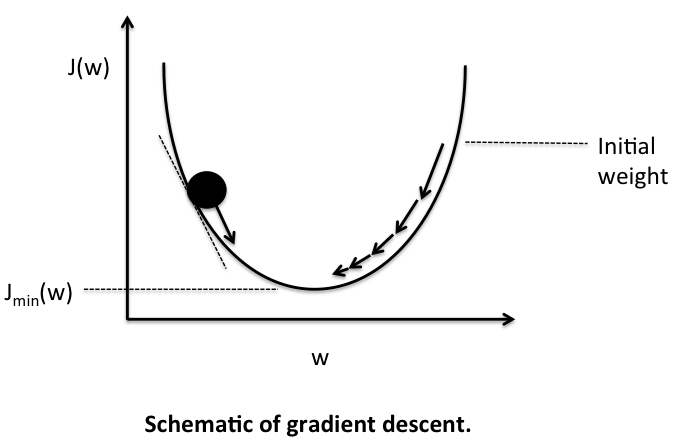
\includegraphics[scale=.2]{graph/gradient_descent}
            \end{figure}
        \end{frame}    
          
        \begin{frame}{objective function}{additive vs.\ multiplicative update rules} 
           optimization of objective function\footfullcite{seung_nmf_2001} $D_\mathrm{EU}( V \parallel WH) = \parallel V - WH\parallel^{2}$
           \begin{itemize}
                \item  \textbf{additive} update rules:
                \begin{equation*}
                H \leftarrow H + \alpha \frac{\partial J}{\partial H} = H + \alpha [(W^{T}V) - (W^{T}WH)]
                \end{equation*}
                \begin{equation*}
                W \leftarrow W + \alpha \frac{\partial J}{\partial W} = W + \alpha [(VH^{T}) - (WHH^{T})]
                \end{equation*}
			   \item<2->  \textbf{multiplicative} update rules:
                \begin{equation*}
                H \leftarrow H \frac{(W^{T}V)}{(W^{T}WH)}
                \end{equation*}
                \begin{equation*}
                W \leftarrow W \frac{(VH^{T})}{(WHH^{T})}
                \end{equation*}
           \end{itemize}
        \end{frame}        
    
        \begin{frame}{objective function}{additional cost function constraints}
            \begin{itemize}
                \item   additional penalty terms (regularization terms) may be added to objective function
                \bigskip
                \item   example: sparsity in $W$ or $H$
                \begin{equation*}
                    D = \parallel V - WH\parallel^{2} + {\color{highlight}{\alpha J_\mathrm{W}(W)}} + {\color{highlight}{\beta J_\mathrm{H}(H)}}
                \end{equation*}
                \begin{itemize}
                    \item $\alpha,\beta$: coefficients for controlling degree of sparsity
                    \item $J_\mathrm{W}$ and $J_\mathrm{H}$: typically $L_{1},L_{2}$ norm 
                \end{itemize}
            \end{itemize}
        \end{frame}
              
    \section[example]{NMF example}
        \begin{frame}{nmf example}{template extraction}
            \vspace{-3mm}
            \begin{columns}
                \column{.4\linewidth}
                    \begin{itemize}
                        \item   unsupervised extraction of templates and activations
                        \item   input audio: 
                            \begin{itemize}
                                \item  \includeaudio{Horn.ff.Db2} horn
                                \item  \includeaudio{Oboe.ff.F4} oboe
                                \item  \includeaudio{Violin.arco.ff.sulD.B4} violin
                                \item  \includeaudio{nmf_mixture} mix
                            \end{itemize}
                    \end{itemize}
                \column{.6\linewidth}
                    \figwithmatlab{F0Nmf}   
            \end{columns}
        \end{frame}
        
        \begin{frame}{nmf use cases}{piano transcription}
            \begin{itemize}
                \item   separate template adaptation from activation matrix adaptation:
                    \begin{enumerate}
                        \item  train/set template matrix
                        \item  order template matrix to have fixed pitch mapping
                        \item  keep template matrix fixed and only update activation matrix
                        \item  pick activation magnitude to determine active pitches
                    \end{enumerate}
                \bigskip
                \item   potential problems
                    \begin{itemize}
                        \item   detuned piano
                        \item   template differs significantly from sound analyzed
                    \end{itemize}
            \end{itemize}
        \end{frame}
        
    \section{summary}
        \begin{frame}{summary}{lecture content}
            \begin{itemize}
                \item   \textbf{polyphonic pitch detection}
                    \begin{itemize}
                        \item   highly challenging task with
                            \begin{itemize}
                                \item   unknown number of sources
                                \item   unknown harmonic structure
                                \item   spectral overlap of sources
                                \item   time-varying mixture
                            \end{itemize}
                    \end{itemize}
                \bigskip
                \item   \textbf{traditional approaches}
                    \begin{itemize}
                        \item   iterative subtraction (detect one pitch, remove it, repeat analysis)
                        \item   multi-band processing
                    \end{itemize}
                \bigskip
                \item   \textbf{non-negative matrix factorization}
                    \begin{itemize}
                        \item   iterative process minimizing an objective function
                        \item   split a matrix into a template matrix and an activation matrix
                    \end{itemize}
           \end{itemize}
            \inserticon{summary}
        \end{frame}
\end{document}
